\subsection{Algoritmer}
%\begin{frame}{Preorder Traversal}
%TODO: Fill with content @Lukas 
%\end{frame}
%
%\begin{frame}{Postorder Traversal}
%TODO: Fill with content @Lukas 
%\end{frame}
%
%\begin{frame}{Inorder Traversal}
%TODO: Fill with content @Lukas 
%\end{frame}

\begin{frame}{Spanning Trees}
	\begin{block}{Spanning Trees}
    Et Spanning Tree for en graf er et tree som besøker alle noder, men ikke lager cycles.
    \end{block}
    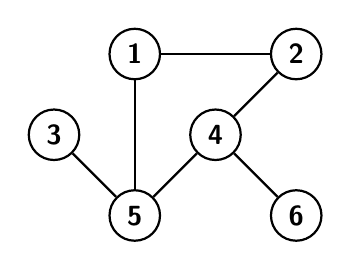
\begin{tikzpicture}[
    node distance=1.45cm, thick,
    main node/.style={circle, draw, font=\sffamily\bfseries}
]
    \node[main node] (1)                    {1};
    \node[main node] (3) [below left  of=1] {3};
    \node[main node] (4) [below right of=1] {4};
    \node[main node] (2) [above right of=4] {2};
    \node[main node] (5) [below right of=3] {5};
    \node[main node] (6) [below right of=4] {6};

    \path (1) edge (2)
        (1) edge (5)
        (3) edge (5)
        (4) edge (2)
        (4) edge (5)
        (4) edge (6);
\end{tikzpicture}
\begin{tikzpicture}[
    node distance=1.45cm, thick,
    main node/.style={circle, draw, font=\sffamily\bfseries}
]
    \node[main node] (1)                    {1};
    \node[main node] (3) [below left  of=1] {3};
    \node[main node] (4) [below right of=1] {4};
    \node[main node] (2) [above right of=4] {2};
    \node[main node] (5) [below right of=3] {5};
    \node[main node] (6) [below right of=4] {6};

    \path (1) edge[properties] (2)
        (1) edge[properties] (5)
        (3) edge[properties] (5)
        (4) edge (2)
        (4) edge[properties] (5)
        (4) edge[properties] (6);
\end{tikzpicture}
\end{frame}

\begin{frame}{Algoritmer for Spanning Trees}
Finne \textit{en} Spanning Tree
\begin{itemize}
\item Breadth-first search (BFS)
\item Depth-first search (DFS)
\end{itemize}
\hspace{1cm}

\noindent Finne \textit{en} Minimum Spanning Tree
\begin{itemize}
\item Prims algoritme
\item Kruskals algoritme
\end{itemize}
\end{frame}

\begin{frame}{BFS og DFS}
\begin{itemize}
\item Begge to går gjennom grafen fra en startnode
\item I hver runde går man videre til naboene til en node
\item Forskjell: BFS bruker kø, DFS stack
\item BFS: Rekkefølgen noder blir markert er rekkefølgen man går gjennom grafen
\item $\rightarrow$ Bredden blir utforsket før
\item DFS: Første noder som blir markiert er siste man ser på
\item $\rightarrow$ Algoritmen søker dypt først
\end{itemize}
\end{frame}

\begin{frame}[fragile]{Breadth-first search (BFS)}
\begin{minted}{python}
def bfs(graph):
   visited = [node] # alle besøkte noder
   queue = [node]   # køen
	
   while queue:     # så lenge noder er igjen
      m = queue.pop(0) # neste node 
      print(f"Visited: {m}")
      for neighbour in graph.neighbours(m): # gå gjennom naboer
         if neighbour not in visited:       # hvis ikke sett før
            visited += neighbour            # add til visited og kø
            queue += neighbour
\end{minted}
\end{frame}

\begin{frame}{Eksempel BFS}
\begin{tikzpicture}[
    node distance=1.45cm, thick,
    main node/.style={circle, draw, font=\sffamily\bfseries}
]
    \node[main node] (1) [onslide=<1->{fill=black!30!red}]                   {1};
    \node[main node] (2) [right of =1,onslide=<2->{fill=black!30!red}] {2};
    \node[main node] (3) [right of =2,onslide=<3->{fill=black!30!red}] {3};
    \node[main node] (4) [right of =3,onslide=<5->{fill=black!30!red}] {4};
    \node[main node] (5) [right of =4,onslide=<6->{fill=black!30!red}] {5};
    \node[main node] (6) [below of =1,onslide=<2->{fill=black!30!red}] {6};
    \node[main node] (7) [right of =6,onslide=<2->{fill=black!30!red}] {7};
    \node[main node] (8) [right of =7,onslide=<3->{fill=black!30!red}] {8};
    \node[main node] (9) [right of =8,onslide=<4->{fill=black!30!red}] {9};
    \node[main node] (0) [right of =9,onslide=<5->{fill=black!30!red}] {0};

    \path (1) edge[onslide=<1->{propertiesBlue},onslide=<2->{propertiesRed}] (2)
        (1) edge[onslide=<1->{propertiesBlue},onslide=<2->{propertiesRed}] (6)
        (1) edge[onslide=<1->{propertiesBlue},onslide=<2->{propertiesRed}] (7)
        (2) edge[onslide=<2->{propertiesBlue},onslide=<3->{propertiesRed}] (3)
        (2) edge[onslide=<2->{propertiesBlue},onslide=<3->{propertiesRed}] (8)
        (3) edge (8)
		(3) edge[onslide=<3->{propertiesBlue},onslide=<4->{propertiesRed}] (9)
        (4) edge[onslide=<4->{propertiesBlue},onslide=<5->{propertiesRed}] (9)
        (9) edge[onslide=<4->{propertiesBlue},onslide=<5->{propertiesRed}] (0)
        (0) edge[onslide=<5->{propertiesBlue},onslide=<6->{propertiesRed}] (5)
        (2) edge (6);
\end{tikzpicture}
\medskip

\only<1>{
	Queue: 2 6 7
}
\only<2>{
	Queue: \cancel{2} \cancel{6} \cancel{7} 3 8
}
\only<3>{
	Queue: \cancel{2} \cancel{6} \cancel{7} \cancel{3} \cancel{8} 9
}
\only<4>{
	Queue: \cancel{2} \cancel{6} \cancel{7} \cancel{3} \cancel{8} \cancel{9} 4 0
}
\only<5>{
	Queue: \cancel{2} \cancel{6} \cancel{7} \cancel{3} \cancel{8} \cancel{9} \cancel{4} \cancel{0} 5
}
\only<6>{
	Queue: \cancel{2} \cancel{6} \cancel{7} \cancel{3} \cancel{8} \cancel{9} \cancel{4} \cancel{0} \cancel{5}
}
\end{frame}

\begin{frame}[fragile]{Depth-first search (DFS)}
\begin{minted}{python}
visited = []	# alle besøkte noder

def dfs(visited, graph, node):
   if node not in visited:      # hvis noden ikke er besøkt
      print(f"Visited: {node}") # markere som besøkt
      visited += node
      
      for neighbour in graph.neighbours(node): # gå gjennom naboer
         dfs(visited, graph, neighbour)        # rekursiv call
\end{minted}
\end{frame}

\begin{frame}{Eksempel DFS}
\begin{tikzpicture}[
    node distance=1.45cm, thick,
    main node/.style={circle, draw, font=\sffamily\bfseries}
]
    \node[main node] (1) [onslide=<1->{fill=black!30!red}]                   {1};
    \node[main node] (2) [right of =1,onslide=<3->{fill=black!30!red}] {2};
    \node[main node] (3) [right of =2,onslide=<4->{fill=black!30!red}] {3};
    \node[main node] (4) [right of =3,onslide=<7->{fill=black!30!red}] {4};
    \node[main node] (5) [right of =4,onslide=<9->{fill=black!30!red}] {5};
    \node[main node] (6) [below of =1,onslide=<11->{fill=black!30!red}] {6};
    \node[main node] (7) [right of =6,onslide=<12->{fill=black!30!red}] {7};
    \node[main node] (8) [right of =7,onslide=<5->{fill=black!30!red}] {8};
    \node[main node] (9) [right of =8,onslide=<6->{fill=black!30!red}] {9};
    \node[main node] (0) [right of =9,onslide=<8->{fill=black!30!red}] {0};

    \path (1) edge[onslide=<2->{propertiesBlue},onslide=<3->{propertiesRed}] (2)
        (1) edge[onslide=<2-11>{propertiesBlue}] (6)
        (1) edge[onslide=<2-11>{propertiesBlue},onslide=<12->{propertiesRed}] (7)
        (2) edge[onslide=<3-3>{propertiesBlue},onslide=<4->{propertiesRed}] (3)
        (2) edge[onslide=<3-9>{propertiesBlue}] (8)
        (3) edge[onslide=<4-5>{propertiesBlue},onslide=<5->{propertiesRed}] (8)
		(3) edge[onslide=<4-5>{propertiesBlue},onslide=<6->{propertiesRed}] (9)
        (4) edge[onslide=<6-6>{propertiesBlue},onslide=<7->{propertiesRed}] (9)
        (9) edge[onslide=<6-7>{propertiesBlue},onslide=<8->{propertiesRed}] (0)
        (0) edge[,onslide=<8-8>{propertiesBlue},onslide=<9->{propertiesRed}] (5)
        (2) edge[onslide=<3-10>{propertiesBlue},onslide=<11->{propertiesRed}] (6);
\end{tikzpicture}
\medskip

\only<1>{
	Stack: 
}
\only<2>{
	Stack: 7 6 2
}
\only<3>{
	Stack: 7 6 \cancel{2} 6 8 3
}
\only<4>{
	Stack: 7 6 \cancel{2} 6 8 \cancel{3} 9 8
}
\only<5>{
	Stack: 7 6 \cancel{2} 6 8 \cancel{3} 9 \cancel{8}
}
\only<6>{
	Stack: 7 6 \cancel{2} 6 8 \cancel{3} \cancel{9} \cancel{8} 0 4
}
\only<7>{
	Stack: 7 6 \cancel{2} 6 8 \cancel{3} \cancel{9} \cancel{8} 0 \cancel{4}
}
\only<8>{
	Stack: 7 6 \cancel{2} 6 8 \cancel{3} \cancel{9} \cancel{8} \cancel{0} \cancel{4} 5
}
\only<9>{
	Stack: 7 6 \cancel{2} 6 8 \cancel{3} \cancel{9} \cancel{8} \cancel{0} \cancel{4} \cancel{5}
}
\only<10>{
	Stack: 7 6 \cancel{2} 6 \cancel{8} \cancel{3} \cancel{9} \cancel{8} \cancel{0} \cancel{4} \cancel{5}
}
\only<11>{
	Stack: 7 6 \cancel{2} \cancel{6} \cancel{8} \cancel{3} \cancel{9} \cancel{8} \cancel{0} \cancel{4} \cancel{5}
}
\only<12>{
	Stack: \cancel{7} \cancel{6} \cancel{2} \cancel{6} \cancel{8} \cancel{3} \cancel{9} \cancel{8} \cancel{0} \cancel{4} \cancel{5}
}
\end{frame}

\begin{frame}{Minimum Spanning Trees}
\begin{block}{Minimum Spanning Trees}
    Et Minimum Spanning Tree for en graf er en Spanning Tree der summen av vektene (weights) er minimal.
    \end{block}
\begin{block}{Kruskals algoritme}
1. Sorter alle kanter etter sine vekter\\
2. Velg kanten med minst vekt som ikke ble valgt før. Hvis det nå blir en syklus, ignorer kanten. Hvis ikke, legg kanten til treet.\\
3. Repeter (2) så lenge til det er (n-1) kanter / alle noder er knyttet sammen.\\
\end{block}
\end{frame}


\begin{frame}{Eksempel Kruskal}
\begin{tikzpicture}[
    node distance=2cm, thick,
    main node/.style={circle, draw, font=\sffamily\bfseries},el/.style = {inner sep=2pt, align=left, sloped},
every label/.append style = {font=\tiny}
]
    \node[main node] (1) [onslide=<3->{fill=black!30!red}] {1};
    \node[main node] (2) [onslide=<3->{fill=black!30!red},right of =1] {2};
    \node[main node] (3) [onslide=<9->{fill=black!30!red},right of =2] {3};
    \node[main node] (4) [onslide=<5->{fill=black!30!red},below right of =1] {4};
    \node[main node] (5) [onslide=<7->{fill=black!30!red},below right of =2] {5};
    \node[main node] (6) [onslide=<15->{fill=black!30!red},below left of =4] {6};
    \node[main node] (7) [onslide=<11->{fill=black!30!red},below right of =4] {7};
    \node[main node] (8) [onslide=<17->{fill=black!30!red},below right of =5] {8};
    
    \path (1)  edge[onslide=<2-2>{propertiesBlue},onslide=<3->{propertiesRed}] node[el,above]  {1}  (2)
     (2)  edge[onslide=<12-12>{propertiesBlue},onslide=<13->{propertiesGrey}] node[el,above]  {5}  (3)
     (1)  edge[onslide=<14-14>{propertiesBlue},onslide=<15->{propertiesRed}] node[el,below]  {5}  (6)
     (2)  edge[onslide=<4-4>{propertiesBlue},onslide=<5->{propertiesRed}] node[el,above]  {2}  (4)
     (2)  edge[onslide=<6-6>{propertiesBlue},onslide=<7->{propertiesRed}] node[el,below]  {3}  (5)
     (3)  edge[onslide=<8-8>{propertiesBlue},onslide=<9->{propertiesRed}] node[el,below]  {4}  (5)
     (5)  edge[onslide=<10-10>{propertiesBlue},onslide=<11->{propertiesRed}] node[el,below]  {4}  (7)
     (3)  edge[onslide=<16-16>{propertiesBlue},onslide=<17->{propertiesRed}] node[el,above]  {8}  (8)
     (6)  edge[onslide=<18->{propertiesGrey}] node[el,below]  {$5,3\cdot 10^{17}$}  (5);
\end{tikzpicture}

\end{frame}